\begin{figure*}[h]
	\centering
	\scriptsize
	%\setlength{\tabcolsep}{5pt}
\begin{tabular}{lrrrrrrrrrrr}
\toprule
      & P1    & P2    & P3    & P4    & P5    & P6    & P7    & P8    & P9    & P10   & P11 \\
\midrule
CP    & \cellcolor{lightgreen}32\%  & \cellcolor{lightred}0\%   & \cellcolor{lightgreen}13\%  & \cellcolor{lightred}0\%   & \cellcolor{lightred}0\%   & \cellcolor{lightred}\cellcolor{lightred}0\%   & \cellcolor{lightred}0\%   & \cellcolor{lightred}0\%   & \cellcolor{lightblack}5\%   & \cellcolor{lightred}0\%   & \cellcolor{lightgreen}50\% \\
CSD   & \cellcolor{lightgreen}32\%  & \cellcolor{lightred}0\%   & \cellcolor{lightgreen}13\%  & \cellcolor{lightred}0\%   & \cellcolor{lightred}0\%   & \cellcolor{lightred}0\%   & \cellcolor{lightred}0\%   & \cellcolor{lightred}0\%   & \cellcolor{lightblack}5\%   & \cellcolor{lightred}0\%   & \cellcolor{lightgreen}50\% \\
DC    & \cellcolor{lightred}0\%   & \cellcolor{lightgreen}32\%  & \cellcolor{lightred}0\%   & \cellcolor{lightgreen}13\%  & \cellcolor{lightred}0\%   & \cellcolor{lightred}0\%   & \cellcolor{lightred}0\%   & \cellcolor{lightred}0\%   & \cellcolor{lightred}0\%   & \cellcolor{lightblack}5\%   & \cellcolor{lightgreen}50\% \\
LIC   & \cellcolor{lightgreen}32\%  & \cellcolor{lightred}0\%   & \cellcolor{lightgreen}13\%  & \cellcolor{lightred}0\%   & \cellcolor{lightred}0\%   & \cellcolor{lightred}0\%   & \cellcolor{lightred}0\%   & \cellcolor{lightred}0\%   & \cellcolor{lightblack}5\%   & \cellcolor{lightred}0\%   & \cellcolor{lightgreen}50\% \\
USA   & \cellcolor{lightgreen}32\%  & \cellcolor{lightred}0\%   & \cellcolor{lightgreen}13\%  & \cellcolor{lightred}0\%   & \cellcolor{lightred}0\%   & \cellcolor{lightred}0\%   & \cellcolor{lightred}0\%   & \cellcolor{lightred}0\%   & \cellcolor{lightblack}5\%   & \cellcolor{lightred}0\%   & \cellcolor{lightgreen}50\% \\
VFR   & \cellcolor{lightgreen}32\%  & \cellcolor{lightred}0\%   & \cellcolor{lightgreen}13\%  & \cellcolor{lightred}0\%   & \cellcolor{lightred}0\%   & \cellcolor{lightred}0\%   & \cellcolor{lightred}0\%   & \cellcolor{lightred}0\%   & \cellcolor{lightblack}5\%   & \cellcolor{lightred}0\%   & \cellcolor{lightgreen}50\% \\
MWN   & \cellcolor{lightgreen}32\%  & \cellcolor{lightred}0\%   & \cellcolor{lightgreen}13\%  & \cellcolor{lightred}0\%   & \cellcolor{lightred}0\%   & \cellcolor{lightred}0\%   & \cellcolor{lightred}0\%   & \cellcolor{lightred}0\%   & \cellcolor{lightblack}5\%   & \cellcolor{lightred}0\%   & \cellcolor{lightgreen}50\% \\
AE    & \cellcolor{lightgreen}65\%  & \cellcolor{lightred}0\%   & \cellcolor{lightgreen}25\%  & \cellcolor{lightred}0\%   & \cellcolor{lightred}0\%   & \cellcolor{lightred}0\%   & \cellcolor{lightred}0\%   & \cellcolor{lightred}0\%   & \cellcolor{lightgreen}10\%  & \cellcolor{lightred}0\%   & \cellcolor{lightred}0\% \\
DOM   & \cellcolor{lightgreen}65\%  & \cellcolor{lightred}0\%   & \cellcolor{lightgreen}25\%  & \cellcolor{lightred}0\%   & \cellcolor{lightblack}7\%   & \cellcolor{lightred}0\%   & \cellcolor{lightblack}2\%   & \cellcolor{lightred}0\%   & \cellcolor{lightred}0\%   & \cellcolor{lightred}0\%   & \cellcolor{lightred}0\% \\
LMA   & \cellcolor{lightgreen}65\%  & \cellcolor{lightred}0\%   & \cellcolor{lightgreen}25\%  & \cellcolor{lightred}0\%   & \cellcolor{lightred}0\%   & \cellcolor{lightred}0\%   & \cellcolor{lightred}0\%   & \cellcolor{lightred}0\%   & \cellcolor{lightgreen}10\%  & \cellcolor{lightred}0\%   & \cellcolor{lightred}0\% \\
LMNA  & \cellcolor{lightgreen}65\%  & \cellcolor{lightred}0\%   & \cellcolor{lightgreen}25\%  & \cellcolor{lightred}0\%   & \cellcolor{lightred}0\%   & \cellcolor{lightred}0\%   & \cellcolor{lightred}0\%   & \cellcolor{lightred}0\%   & \cellcolor{lightgreen}10\%  & \cellcolor{lightred}0\%   & \cellcolor{lightred}0\% \\
LV   & \cellcolor{lightred}0\%   & \cellcolor{lightgreen}65\%  & \cellcolor{lightred}0\%   & \cellcolor{lightgreen}25\%  & \cellcolor{lightred}0\%   & \cellcolor{lightred}0\%   & \cellcolor{lightred}0\%   & \cellcolor{lightred}0\%   & \cellcolor{lightred}0\%   & \cellcolor{lightgreen}10\%  & \cellcolor{lightred}0\% \\
NA    & \cellcolor{lightgreen}65\%  & \cellcolor{lightred}0\%   & \cellcolor{lightgreen}25\%  & \cellcolor{lightred}0\%   & \cellcolor{lightred}0\%   & \cellcolor{lightred}0\%   & \cellcolor{lightred}0\%   & \cellcolor{lightred}0\%   & \cellcolor{lightgreen}10\%  & \cellcolor{lightred}0\%   & \cellcolor{lightred}0\% \\
PDOM  & \cellcolor{lightred}0\%   & \cellcolor{lightgreen}65\%  & \cellcolor{lightred}0\%   & \cellcolor{lightgreen}25\%  & \cellcolor{lightred}0\%   & \cellcolor{lightblack}7\%   & \cellcolor{lightred}0\%   & \cellcolor{lightblack}2\%   & \cellcolor{lightred}0\%   & \cellcolor{lightred}0\%   & \cellcolor{lightred}0\% \\
RD    & \cellcolor{lightgreen}65\%  & \cellcolor{lightred}0\%   & \cellcolor{lightgreen}25\%  & \cellcolor{lightred}0\%   & \cellcolor{lightred}0\%   & \cellcolor{lightred}0\%   & \cellcolor{lightred}0\%   & \cellcolor{lightred}0\%   & \cellcolor{lightgreen}10\%  & \cellcolor{lightred}0\%   & \cellcolor{lightred}0\% \\
RS    & \cellcolor{lightgreen}65\%  & \cellcolor{lightred}0\%   & \cellcolor{lightgreen}25\%  & \cellcolor{lightred}0\%   & \cellcolor{lightred}0\%   & \cellcolor{lightred}0\%   & \cellcolor{lightred}0\%   & \cellcolor{lightred}0\%   & \cellcolor{lightgreen}10\%  & \cellcolor{lightred}0\%   & \cellcolor{lightred}0\% \\
VBE   & \cellcolor{lightred}0\%   & \cellcolor{lightgreen}65\%  & \cellcolor{lightred}0\%   & \cellcolor{lightgreen}25\%  & \cellcolor{lightred}0\%   & \cellcolor{lightred}0\%   & \cellcolor{lightred}0\%   & \cellcolor{lightred}0\%   & \cellcolor{lightred}0\%   & \cellcolor{lightgreen}10\%  & \cellcolor{lightred}0\% \\
SS    & \cellcolor{lightgreen}65\%  & \cellcolor{lightred}0\%   & \cellcolor{lightgreen}25\%  & \cellcolor{lightred}0\%   & \cellcolor{lightred}0\%   & \cellcolor{lightred}0\%   & \cellcolor{lightred}0\%   & \cellcolor{lightred}0\%   & \cellcolor{lightgreen}10\%  & \cellcolor{lightred}0\%   & \cellcolor{lightred}0\% \\
UDV   & \cellcolor{lightred}0\%   & \cellcolor{lightred}0\%   & \cellcolor{lightred}0\%   & \cellcolor{lightred}0\%   & \cellcolor{lightred}0\%   & \cellcolor{lightred}0\%   & \cellcolor{lightred}0\%   & \cellcolor{lightred}0\%   & \cellcolor{lightred}0\%   & \cellcolor{lightred}0\%   & \cellcolor{lightgreen}100\% \\
UIR   & \cellcolor{lightred}0\%   & \cellcolor{lightred}0\%   & \cellcolor{lightred}0\%   & \cellcolor{lightred}0\%   & \cellcolor{lightred}0\%   & \cellcolor{lightred}0\%   & \cellcolor{lightred}0\%   & \cellcolor{lightred}0\%   & \cellcolor{lightred}0\%   & \cellcolor{lightred}0\%   & \cellcolor{lightgreen}100\% \\
WNIL  & \cellcolor{lightred}0\%   & \cellcolor{lightred}0\%   & \cellcolor{lightred}0\%   & \cellcolor{lightred}0\%   & \cellcolor{lightred}0\%   & \cellcolor{lightred}0\%   & \cellcolor{lightred}0\%   & \cellcolor{lightred}0\%   & \cellcolor{lightred}0\%   & \cellcolor{lightred}0\%   & \cellcolor{lightgreen}100\% \\
\midrule
Overall & \cellcolor{lightgreen}32.46\% & \cellcolor{lightgreen}9.27\% & \cellcolor{lightgreen}12.69\% & \cellcolor{lightblack}3.62\% & \cellcolor{lightblue}0.26\% & \cellcolor{lightblue}0.26\% & \cellcolor{lightblue}0.10\% & \cellcolor{lightblue}0.10\% & \cellcolor{lightblack}4.50\% & \cellcolor{lightblack}1.04\% & \cellcolor{lightgreen}35.70\% \\
\bottomrule
\end{tabular}%
	\caption{Distribution of decisions over the paths of the decision tree for the DaCapo Dataset.}
	\label{fig:paths-dacapo}
\end{figure*}

%\begin{table}%
%\centering
%\scriptsize
%\caption{Reduction in running times. Background colors indicate the ranges of 
%values: \colorbox{lightred}{0\%}, \colorbox{lightblue}{(0\%, 1\%)}, 
%\colorbox{lightblack}{[1\%, 10\%)} and \colorbox{lightgreen}{[10\%, 100\%]}.}
%\begin{tabular}{lrrrrrrrrrrr}
%\toprule
      %& P1    & P2    & P3    & P4    & P5    & P6    & P7    & P8    & P9    & P10   & P11 \\
%\midrule
%CP    & 32\%  & 0\%   & 13\%  & 0\%   & 0\%   & 0\%   & 0\%   & 0\%   & 5\%   & 0\%   & 50\% \\
%CSD   & 32\%  & 0\%   & 13\%  & 0\%   & 0\%   & 0\%   & 0\%   & 0\%   & 5\%   & 0\%   & 50\% \\
%DC    & 0\%   & 32\%  & 0\%   & 13\%  & 0\%   & 0\%   & 0\%   & 0\%   & 0\%   & 5\%   & 50\% \\
%USA   & 22\%  & 0\%   & 8\%   & 0\%   & 0\%   & 0\%   & 0\%   & 0\%   & 3\%   & 0\%   & 67\% \\
%AE    & 65\%  & 0\%   & 25\%  & 0\%   & 0\%   & 0\%   & 0\%   & 0\%   & 10\%  & 0\%   & 0\% \\
%Dom   & 65\%  & 0\%   & 25\%  & 0\%   & 7\%   & 0\%   & 2\%   & 0\%   & 0\%   & 0\%   & 0\% \\
%LIC   & 22\%  & 0\%   & 8\%   & 0\%   & 0\%   & 0\%   & 0\%   & 0\%   & 3\%   & 0\%   & 67\% \\
%LMA   & 65\%  & 0\%   & 25\%  & 0\%   & 0\%   & 0\%   & 0\%   & 0\%   & 10\%  & 0\%   & 0\% \\
%LMNA  & 65\%  & 0\%   & 25\%  & 0\%   & 0\%   & 0\%   & 0\%   & 0\%   & 10\%  & 0\%   & 0\% \\
%LV    & 0\%   & 2\%   & 0\%   & 97\%  & 0\%   & 0\%   & 0\%   & 0\%   & 0\%   & 0\%   & 0\% \\
%NA    & 65\%  & 0\%   & 25\%  & 0\%   & 0\%   & 0\%   & 0\%   & 0\%   & 10\%  & 0\%   & 0\% \\
%PDOM  & 0\%   & 65\%  & 0\%   & 25\%  & 0\%   & 7\%   & 0\%   & 2\%   & 0\%   & 0\%   & 0\% \\
%RD    & 65\%  & 0\%   & 25\%  & 0\%   & 0\%   & 0\%   & 0\%   & 0\%   & 10\%  & 0\%   & 0\% \\
%RS    & 65\%  & 0\%   & 25\%  & 0\%   & 0\%   & 0\%   & 0\%   & 0\%   & 10\%  & 0\%   & 0\% \\
%VBE   & 0\%   & 65\%  & 0\%   & 25\%  & 0\%   & 0\%   & 0\%   & 0\%   & 0\%   & 10\%  & 0\% \\
%UDV   & 0\%   & 0\%   & 0\%   & 0\%   & 0\%   & 0\%   & 0\%   & 0\%   & 0\%   & 0\%   & 100\% \\
%UIR   & 0\%   & 0\%   & 0\%   & 0\%   & 0\%   & 0\%   & 0\%   & 0\%   & 0\%   & 0\%   & 100\% \\
%WNIL  & 0\%   & 0\%   & 0\%   & 0\%   & 0\%   & 0\%   & 0\%   & 0\%   & 0\%   & 0\%   & 100\% \\
%\midrule
%Overall & 13.99\% & 5.09\% & 5.47\% & 53.01\% & 0.14\% & 0.14\% & 0.05\% & 0.05\% & 1.90\% & 0.57\% & 19.59\% \\
%\bottomrule
%\end{tabular}%
%\label{tab:decision-distribution}
%\end{table}

%\begin{figure}[!t]
	%\centering
	%\subfloat[DaCapo] {
		%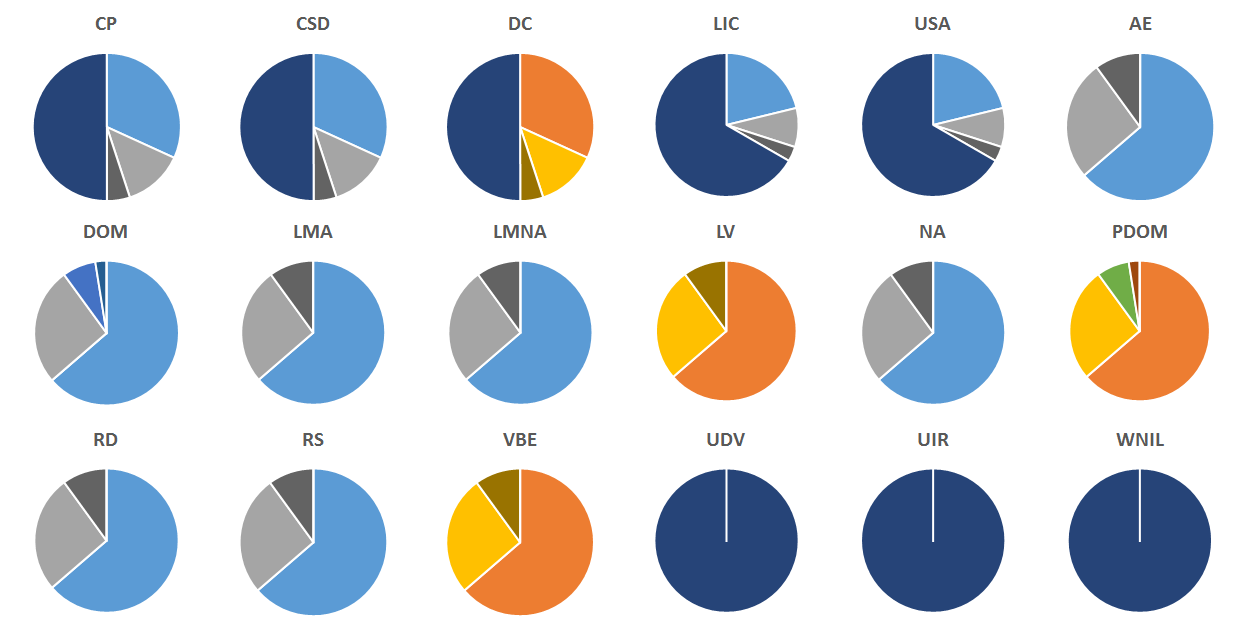
\includegraphics[width=0.8\linewidth]{ecoop-figures/distribution-decision-dacapo.png}
		%\label{fig:paths-dacapo}
	%}\\
	%\subfloat[SourceForge] {
	%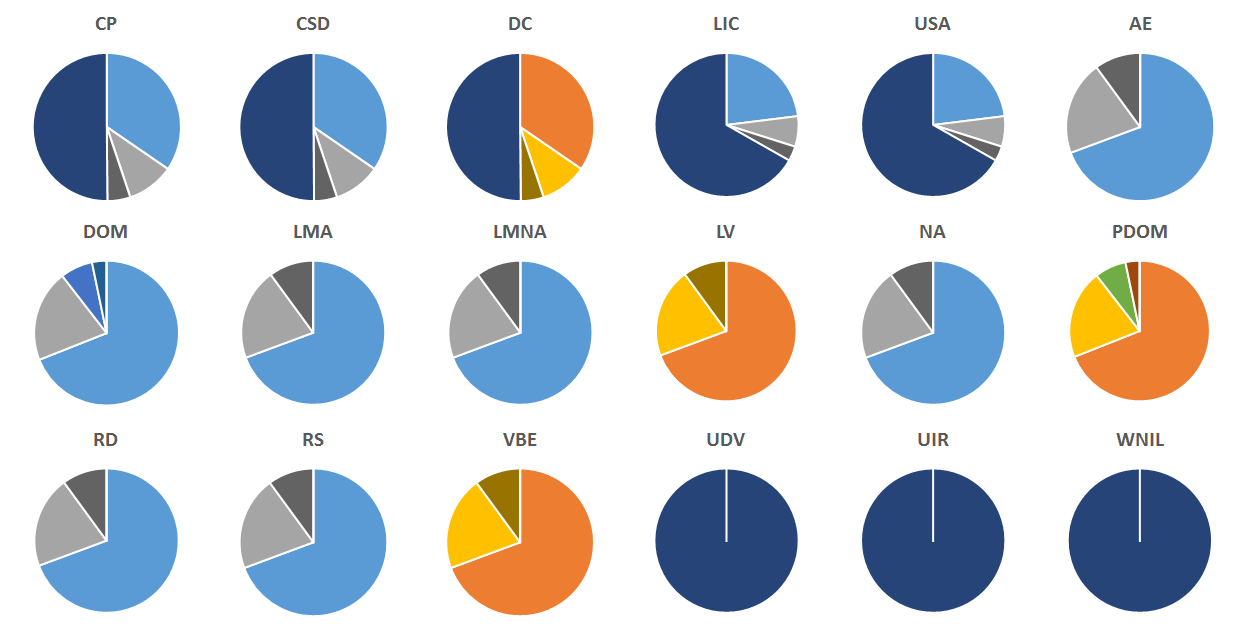
\includegraphics[width=0.8\linewidth]{ecoop-figures/distribution-decision-sf.png}
		%\label{fig:paths-sf}
	%}\\
	%\subfloat[All analyses] {
	%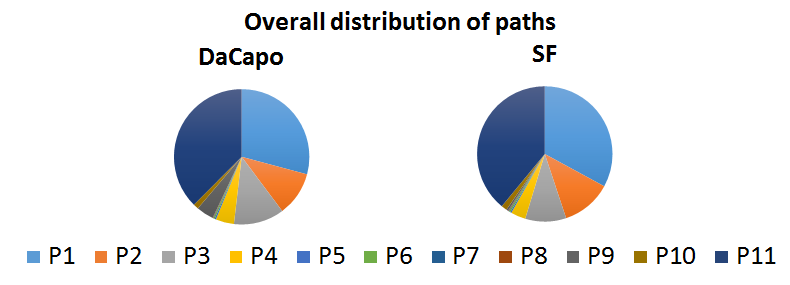
\includegraphics[width=0.8\linewidth]{ecoop-figures/distribution-decision-overall.png}
		%\label{fig:paths-all}
	%}
	%\caption{Distribution of decisions over the paths of the decision tree.}
	%\label{fig:decision-distribution}
%\end{figure}
